\begin{figure}[H]
    \begin{center}
        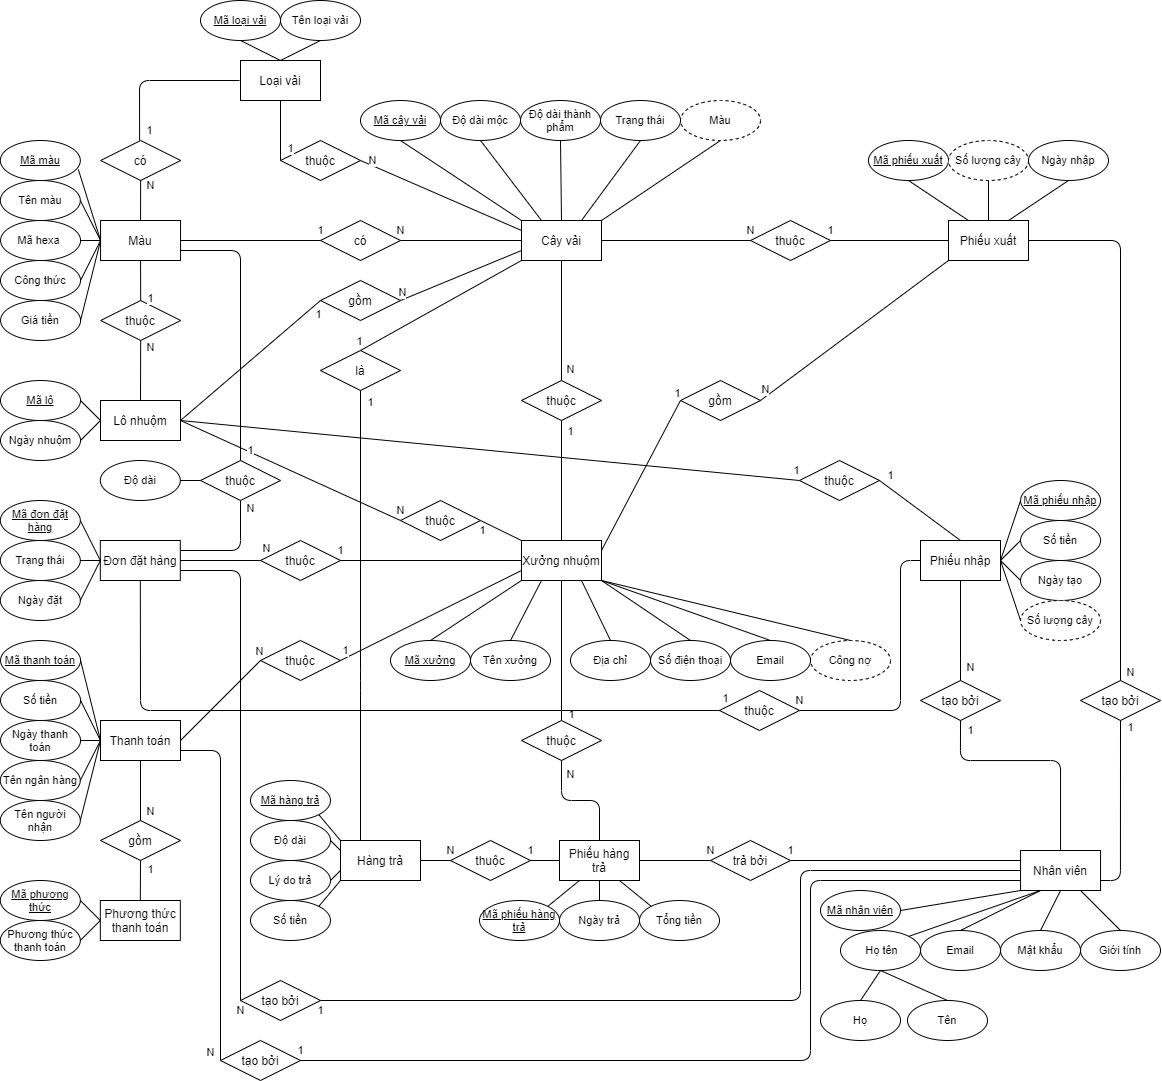
\includegraphics[width=17cm]{Image/General/ERD.png}
        \caption{Mô hình ERD của hệ thống}
        \label{erd}
    \end{center}
\end{figure}
\newpage
Cơ sở dữ liệu của hệ thống được thiết kế dựa trên mô hình  ERD như Hình \ref{erd}

Từ mô hình trên ánh xạ ra mô hình CSDL quan hệ với các bảng được mô tả trong Hình \ref{relation_model}.

\begin{figure}[H]
    \begin{center}
        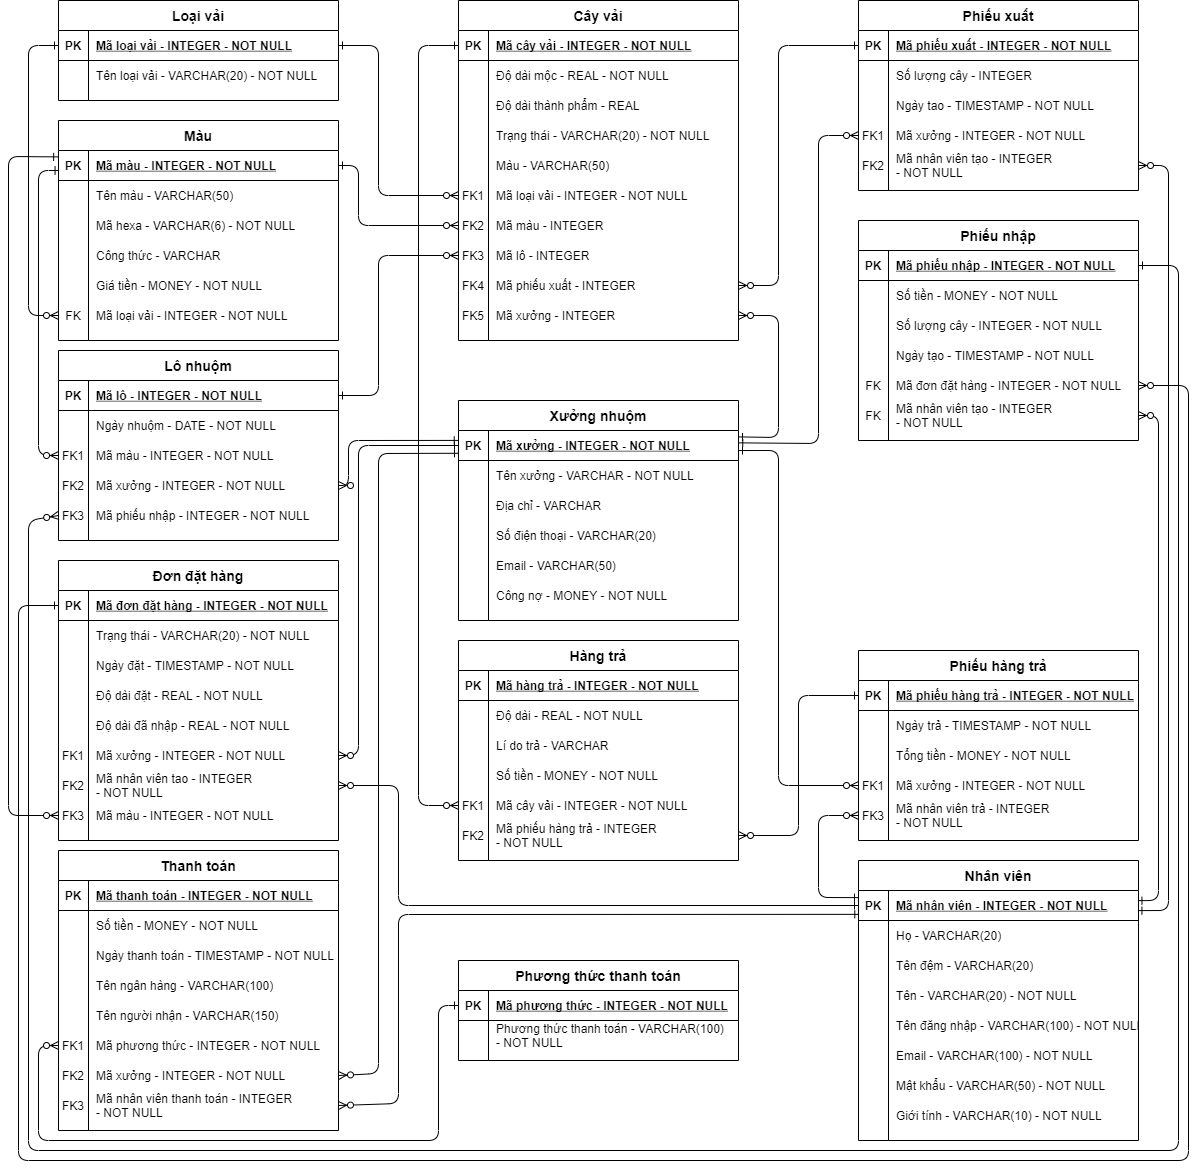
\includegraphics[width=17cm]{Image/General/Relational Data Model.png}
        \caption{Mô hình CSDL quan hệ của hệ thống}
        \label{relation_model}
    \end{center}
\end{figure}

\newpage
Sau khi thiết kế ERD nhóm tiến hành chuyển đổi thành các bảng tương ứng trong database như sau:
\begin{itemize}
    \item \textbf{fabric\_type}
    \begin{table}[H]
        \centering
        \begin{tabular}{|m{3cm}|m{10cm}|}
        \hline 
            id & Mã loại vải\\ \hline
            type & Kí hiệu loại vải \\ \hline
            name & Tên loại vải\\
        \hline 
        \end{tabular}
        \caption{Loại vải}
        \label{fabric_type}
    \end{table}
    
    \item \textbf{color}
    \begin{table}[H]
        \centering
        \begin{tabular}{|m{3cm}|m{10cm}|}
        \hline 
            id & Mã màu\\ \hline
            type & Kí hiệu màu \\ \hline
            name & Tên màu\\ \hline
            hexa\_code & Mã hexa của màu \\ \hline
            recipe & Công thức để thực hiện màu \\ \hline
            price & Giá tiền thi công nhuộm của loại vải và màu tương ứng \\ \hline
            fabric\_type\_id & Mã loại vải \\ 
        \hline 
        \end{tabular}
        \caption{Màu}
        \label{color}
    \end{table}
    
    \item \textbf{dyehouse}
    \begin{table}[H]
        \centering
        \begin{tabular}{|m{3cm}|m{10cm}|}
        \hline 
            id & Mã xưởng nhuộm\\ \hline
            name & Tên xưởng nhuộm \\ \hline
            address & Địa chỉ của xưởng nhuộm\\ \hline
            phone\_number & Số điện thoại của xưởng nhuộm \\ \hline
            email & Email của xưởng nhuộm\\ \hline
            debt & Công nợ hiện tại của xưởng nhuộm\\
        \hline 
        \end{tabular}
        \caption{Xưởng nhuộm}
        \label{dyehouse}
    \end{table}
    
    \item \textbf{users}
    \begin{table}[H]
        \centering
        \begin{tabular}{|m{3cm}|m{10cm}|}
        \hline 
            id & Mã người dùng\\ \hline
            first\_name & Họ người dùng \\ \hline
            last\_name & Tên người dùng\\ \hline
            email & Email của người dùng, tên đăng nhập của tài khoản \\ \hline
            password & Password của tài khoản\\ \hline
            sex & Giới tính của người dùng\\
        \hline 
        \end{tabular}
        \caption{Người dùng}
        \label{users}
    \end{table}
    
    \newpage
    \item \textbf{roles}
    \begin{table}[H]
        \centering
        \begin{tabular}{|m{3cm}|m{10cm}|}
        \hline 
            id & Mã vai trò\\ \hline
            name & Tên vai trò\\
        \hline 
        \end{tabular}
        \caption{Vai trò}
        \label{roles}
    \end{table}
    
    \item \textbf{users\_roles}
    \begin{table}[H]
        \centering
        \begin{tabular}{|m{3cm}|m{10cm}|}
        \hline 
            id & Mã người dùng - vai trò\\ \hline
            users\_id & Mã người dùng\\ \hline
            roles\_id & Mã vai trò\\
        \hline 
        \end{tabular}
        \caption{Người dùng - Vai trò}
        \label{users_roles}
    \end{table}
    
    \item \textbf{persistent\_login}
    \begin{table}[H]
        \centering
        \begin{tabular}{|m{3cm}|m{10cm}|}
        \hline 
            id & Mã persistent login\\ \hline
            user\_id & Mã người dùng\\ \hline
            token & Mã token\\ \hline
            last\_update & Thời gian cập nhận lần cuối\\
        \hline 
        \end{tabular}
        \caption{Persistent login}
        \label{persistent_login}
    \end{table}
    
    \item \textbf{orders}
    \begin{table}[H]
        \centering
        \begin{tabular}{|m{3cm}|m{10cm}|}
        \hline 
            id & Mã đơn đặt hàng\\ \hline
            status & Trạng thái đơn đặt hàng \\ \hline
            create\_date & Ngày tạo đơn đặt hàng \\ \hline
            order\_length & Độ dài đặt\\ \hline
            done\_length & Độ dài thành phẩm\\ \hline
            dyehouse\_id & Mã xưởng nhuộm\\ \hline
            user\_id & Mã người dùng\\ \hline
            color\_id & Mã màu\\
        \hline 
        \end{tabular}
        \caption{Đơn đặt hàng}
        \label{orders}
    \end{table}
    
    \item \textbf{import\_slip}
    \begin{table}[H]
        \centering
        \begin{tabular}{|m{3cm}|m{10cm}|}
        \hline 
            id & Mã phiếu nhập\\ \hline
            money & Số tiền tương ứng với phiếu nhập \\ \hline
            fabric\_number & Số lượng cây vải\\ \hline
            create\_date & Ngày tạo phiếu nhập \\ \hline
            order\_id & Mã đơn đặt hàng\\ \hline
            user\_id & Mã người dùng\\ \hline
            driver & Tên tài xế nhập hàng\\
        \hline 
        \end{tabular}
        \caption{Phiếu nhập}
        \label{import_slip}
    \end{table}
    
    \newpage
    \item \textbf{export\_slip}
    \begin{table}[H]
        \centering
        \begin{tabular}{|m{3cm}|m{10cm}|}
        \hline 
            id & Mã phiếu xuất\\ \hline
            fabric\_number & Số lượng cây vải\\ \hline
            create\_date & Ngày tạo phiếu xuất \\ \hline
            dyehouse\_id & Mã xưởng nhuộm\\ \hline
            user\_id & Mã người dùng\\ 
        \hline 
        \end{tabular}
        \caption{Phiếu xuất}
        \label{export_slip}
    \end{table}
    
    \item \textbf{dye\_batch}
    \begin{table}[H]
        \centering
        \begin{tabular}{|m{3cm}|m{10cm}|}
        \hline 
            id & Mã lô nhuộm\\ \hline
            dye\_date & Ngày nhuộm\\ \hline
            color\_id & Mã màu \\ \hline
            dyehouse\_id & Mã xưởng nhuộm\\ \hline
            import\_slip\_id & Mã phiếu nhập\\ 
        \hline 
        \end{tabular}
        \caption{Lô nhuộm}
        \label{dye_batch}
    \end{table}
    
    \item \textbf{payment\_method}
    \begin{table}[H]
        \centering
        \begin{tabular}{|m{3cm}|m{10cm}|}
        \hline 
            id & Mã phương thức thanh toán\\ \hline
            name & Tên phương thức thanh toán\\ 
        \hline 
        \end{tabular}
        \caption{Phương thức thanh toán}
        \label{payment_method}
    \end{table}
    
    \item \textbf{payment}
    \begin{table}[H]
        \centering
        \begin{tabular}{|m{3.5cm}|m{10cm}|}
        \hline 
            id & Mã thanh toán\\ \hline
            money & Số tiền thanh toán\\ \hline
            create\_date & Ngày thanh toán \\ \hline
            bank\_name & Tên ngân hàng\\ \hline
            recipient\_name & Người nhận thanh toán\\ \hline
            payment\_method\_id & Phương thức thanh toán \\ \hline
            dyehouse\_id & Mã xưởng nhuộm\\ \hline
            user\_id & Mã người dùng\\ 
        \hline 
        \end{tabular}
        \caption{Thanh toán}
        \label{payment}
    \end{table}
    
    \newpage
    \item \textbf{fabric}
    \begin{table}[H]
        \centering
        \begin{tabular}{|m{3cm}|m{10cm}|}
        \hline 
            id & Mã cây vải\\ \hline
            raw\_length & Độ dài thô\\ \hline
            finished\_length & Độ dài thành phẩm \\ \hline
            status & Trạng thái của cây vải\\ \hline
            color\_name & Tên màu\\ \hline
            fabric\_type\_id & Mã loại vải\\ \hline
            color\_id & Mã màu \\ \hline
            dye\_batch\_id & Mã lô nhuộm\\ \hline
            export\_slip\_id & Mã phiếu xuất\\ \hline
            dyehouse\_id & Mã xưởng nhuộm\\ 
        \hline 
        \end{tabular}
        \caption{Cây vải}
        \label{fabric}
    \end{table}

    \item \textbf{return\_slip}
    \begin{table}[H]
        \centering
        \begin{tabular}{|m{3cm}|m{10cm}|}
        \hline 
            id & Mã phiếu hàng trả\\ \hline
            return\_date & Ngày tạo phiếu hàng trả\\ \hline
            money & Số tiền tương ứng với phiếu hàng trả \\ \hline
            received\_name & Tên người nhận hàng trả\\ \hline
            dyehouse\_id & Mã xưởng nhuộm\\ \hline
            user\_id & Mã người dùng\\ 
        \hline 
        \end{tabular}
        \caption{Phiếu hàng trả}
        \label{return_slip}
    \end{table}
    
    \item \textbf{returns}
    \begin{table}[H]
        \centering
        \begin{tabular}{|m{3cm}|m{10cm}|}
        \hline 
            id & Mã hàng trả\\ \hline
            return\_length & Độ dài trả\\ \hline
            return\_reason & Lí do trả \\ \hline
            money & Số tiền tương ứng với hàng trả\\ \hline
            fabric\_id & Mã cây vải\\ \hline
            return\_slip\_id & Mã phiếu hàng trả\\ 
        \hline 
        \end{tabular}
        \caption{Hàng trả}
        \label{returns}
    \end{table}


\end{itemize}


\newpage